% --------------------------------------------------------------------------- %
% Poster for the ECCS 2011 Conference about Elementary Dynamic Networks.      %
% --------------------------------------------------------------------------- %
% Created with Brian Amberg's LaTeX Poster Template. Please refer for the     %
% attached README.md file for the details how to compile with `pdflatex`.     %
% --------------------------------------------------------------------------- %
% $LastChangedDate:: 2011-09-11 10:57:12 +0200 (V, 11 szept. 2011)          $ %
% $LastChangedRevision:: 128                                                $ %
% $LastChangedBy:: rlegendi                                                 $ %
% $Id:: poster.tex 128 2011-09-11 08:57:12Z rlegendi                        $ %
% --------------------------------------------------------------------------- %
%\documentclass[a0paper,portrait]{baposter}
\documentclass[fpga_paper,portrait]{baposter}

\usepackage{relsize}		% For \smaller
\usepackage{url}			% For \url
\usepackage{epstopdf}	% Included EPS files automatically converted to PDF to include with pdflatex

%%% Global Settings %%%%%%%%%%%%%%%%%%%%%%%%%%%%%%%%%%%%%%%%%%%%%%%%%%%%%%%%%%%

\graphicspath{{pix/}}	% Root directory of the pictures 
\tracingstats=2			% Enabled LaTeX logging with conditionals

%%% Color Definitions %%%%%%%%%%%%%%%%%%%%%%%%%%%%%%%%%%%%%%%%%%%%%%%%%%%%%%%%%

\definecolor{bordercol}{RGB}{40,40,40}
\definecolor{headercol1}{RGB}{186,215,230}
\definecolor{headercol2}{RGB}{80,80,80}
\definecolor{headerfontcol}{RGB}{0,0,0}
\definecolor{boxcolor}{RGB}{186,215,230}

%%%%%%%%%%%%%%%%%%%%%%%%%%%%%%%%%%%%%%%%%%%%%%%%%%%%%%%%%%%%%%%%%%%%%%%%%%%%%%%%
%%% Utility functions %%%%%%%%%%%%%%%%%%%%%%%%%%%%%%%%%%%%%%%%%%%%%%%%%%%%%%%%%%

%%% Save space in lists. Use this after the opening of the list %%%%%%%%%%%%%%%%
\newcommand{\compresslist}{
	\setlength{\itemsep}{1pt}
	\setlength{\parskip}{0pt}
	\setlength{\parsep}{0pt}
}

%%%%%%%%%%%%%%%%%%%%%%%%%%%%%%%%%%%%%%%%%%%%%%%%%%%%%%%%%%%%%%%%%%%%%%%%%%%%%%%
%%% Document Start %%%%%%%%%%%%%%%%%%%%%%%%%%%%%%%%%%%%%%%%%%%%%%%%%%%%%%%%%%%%
%%%%%%%%%%%%%%%%%%%%%%%%%%%%%%%%%%%%%%%%%%%%%%%%%%%%%%%%%%%%%%%%%%%%%%%%%%%%%%%

\begin{document}
\typeout{Poster rendering started}

%%% Setting Background Image %%%%%%%%%%%%%%%%%%%%%%%%%%%%%%%%%%%%%%%%%%%%%%%%%%
\background{
	\begin{tikzpicture}[remember picture,overlay]%
	\draw (current page.north west)+(-2em,2em) node[anchor=north west]
	{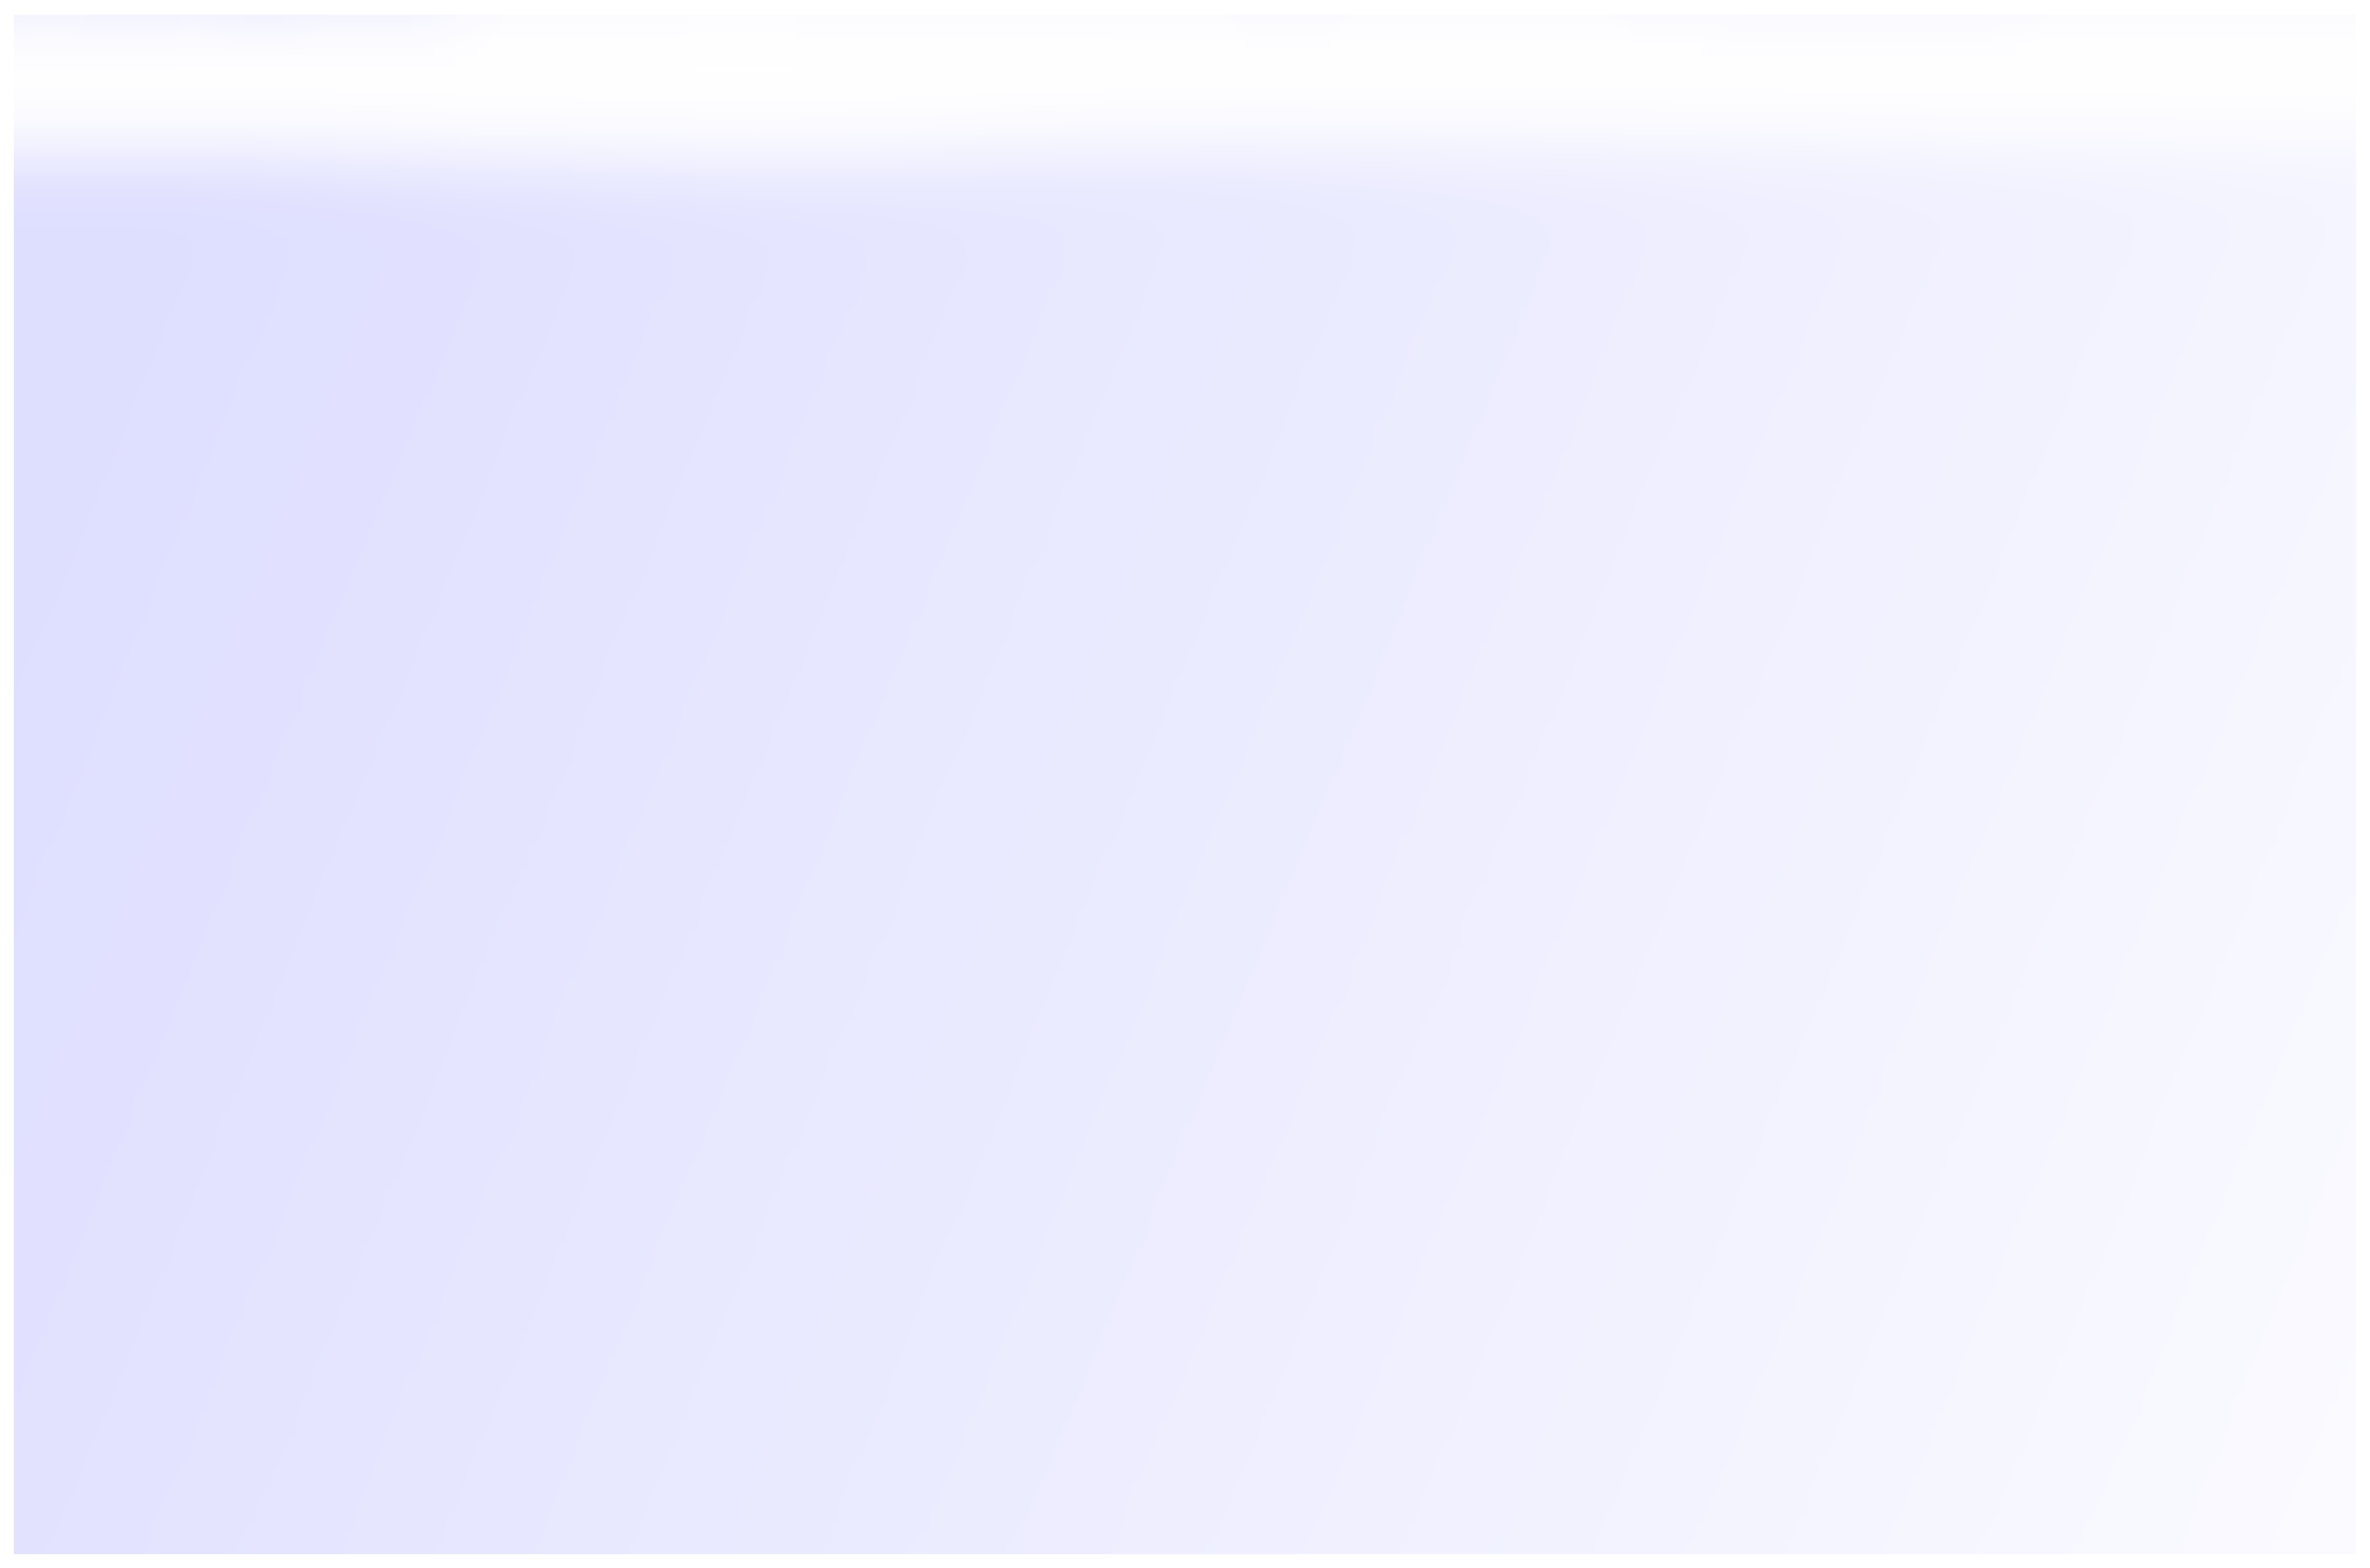
\includegraphics[height=1.1\textheight]{background}};
	\end{tikzpicture}
}

%%% General Poster Settings %%%%%%%%%%%%%%%%%%%%%%%%%%%%%%%%%%%%%%%%%%%%%%%%%%%
%%%%%% Eye Catcher, Title, Authors and University Images %%%%%%%%%%%%%%%%%%%%%%
\begin{poster}{
	grid=false,
	% Option is left on true though the eyecatcher is not used. The reason is
	% that we have a bit nicer looking title and author formatting in the headercol
	% this way
	%eyecatcher=false, 
	borderColor=bordercol,
	headerColorOne=headercol1,
	headerColorTwo=headercol2,
	headerFontColor=headerfontcol,
	% Only simple background color used, no shading, so boxColorTwo isn't necessary
	boxColorOne=boxcolor,
	headershape=roundedright,
	headerfont=\Large\sf\bf,
	textborder=rectangle,
	background=user,
	headerborder=open,
  boxshade=plain
}
%%% Eye Cacther %%%%%%%%%%%%%%%%%%%%%%%%%%%%%%%%%%%%%%%%%%%%%%%%%%%%%%%%%%%%%%%
{
	Eye Catcher, empty if option eyecatcher=false - unused
}
%%% Title %%%%%%%%%%%%%%%%%%%%%%%%%%%%%%%%%%%%%%%%%%%%%%%%%%%%%%%%%%%%%%%%%%%%%
{\huge\sf\bf
	FPGA-based Nintendo Entertainment Systems
}
%%% Authors %%%%%%%%%%%%%%%%%%%%%%%%%%%%%%%%%%%%%%%%%%%%%%%%%%%%%%%%%%%%%%%%%%%
{
	\vspace{1em} Zhi Liu, Yihe Zhang, Qiang Wan, Junjian Xie\\
	{\smaller zhiliu@andrew.cmu.edu, yihez@andrew.cmu.edu, \\qiangwan@andrew.cmu.edu, junjianx@andrew.cmu.edu}
}
%%% Logo %%%%%%%%%%%%%%%%%%%%%%%%%%%%%%%%%%%%%%%%%%%%%%%%%%%%%%%%%%%%%%%%%%%%%%
{
% The logos are compressed a bit into a simple box to make them smaller on the result
% (Wasn't able to find any bigger of them.)
\setlength\fboxsep{0pt}
\setlength\fboxrule{0.5pt}
	\fbox{
		\begin{minipage}{14em}
	%		
\includegraphics[width=10em,height=4em]{colbud_logo}
			
\includegraphics[width=4em,height=4em]{jie_log.png} 
			
\includegraphics[width=10em,height=4em]{jie.png} \\
			
\includegraphics[width=14em,height=4em]{ece_logo}
	%		\includegraphics[width=4em,height=4em]{aitia_logo}
		\end{minipage}
	}
}

\headerbox{Background}{name=background,column=0,row=0}{
	Nintendo Entertainment System(NES) is the platform of many famous games, such as Super Mario, Contra and Tank1990. The aim of our project is to build a NES on FPGA using SystemVerilog, Particularly, we'd implemented major components of the game Tank1990.
\begin{center}
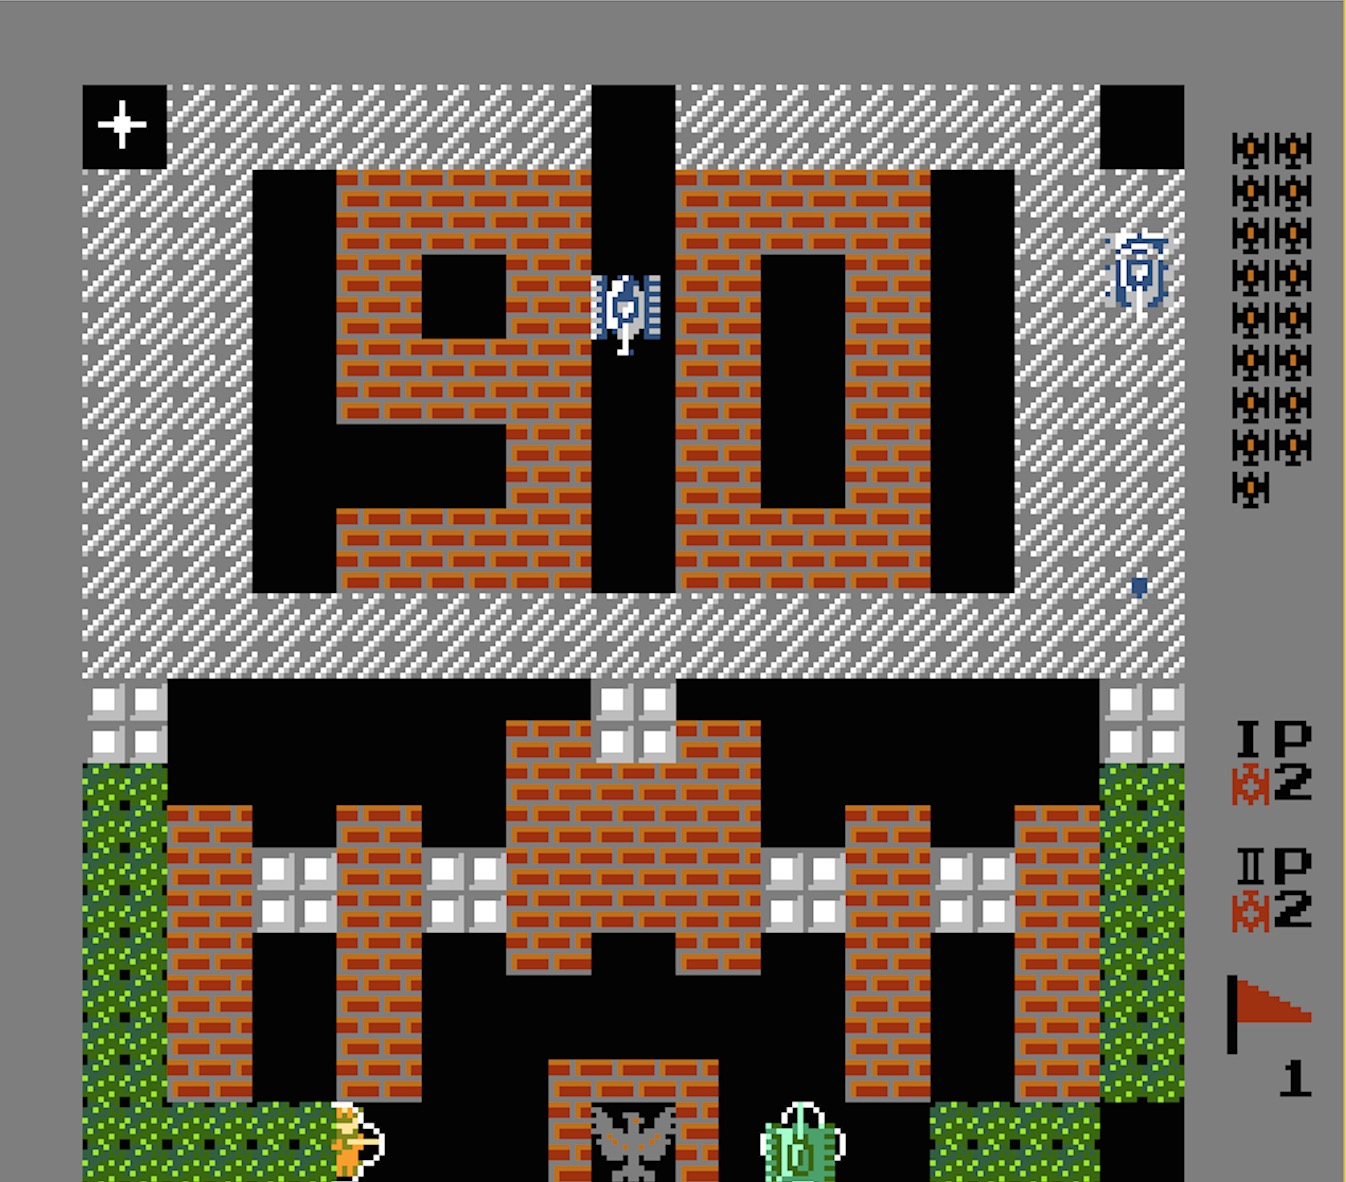
\includegraphics[width=0.66\linewidth]{tank90.png}
\end{center}
%\includegraphics[width=\linewidth]{time_windows}

}


\headerbox{Prep Work}{name=prep_work,column=0,below=background}{
Before we start to build the NES on the FPGA, we decided to write an emulator in C++ at first, because we couldn't begin to debug the problem until we understood how the chip worked and it turn out to be effective and necessary.
}

\headerbox{Basic Concepts}{name=definitions,column=0,below=prep_work}{
\textbf{FSM} is conceived as an abstract machine that can be in one of a finite number of states. The machine is in only one state at a time, it can change from one state to another when initiated by a triggering event or condition. \\
\textbf{CPU6502} is a 8bit Data-16bit Address CPU, accumulator based processor with multiple instruction lengths. There are 3 interrupt methods, 5 program visible registers(an 8bit Accumulator which performs math operations, two 8bit addressing registers X and Y, an 8 bit Stack register for subroutines and interrupt handlers, and a 16 bit Program Counter).
\\
\textbf{PPU} is known for its effective use of memory, using very little memory to store graphical data. \\
}


%\headerbox{PmodJSTK}{name=joystick,column=0,below=acknowledgements, above=bottom}{
\headerbox{PmodJSTK}{name=joystick,column=0,below=definitions}{
The PmodJSTK contains a resistive twin axis joystick that includes a center push button along with two additional push buttons. Also, PmodJSTK has two programmable LEDs located on the board that can provide additional information to the user.\\
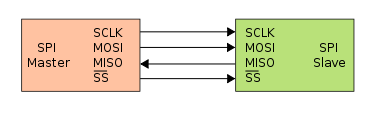
\includegraphics[width=1.0\linewidth]{spi_master_slave}
The serial peripheral interface (SPI) mode 0 method of communication is used to communicate between the PmodJSTK and the master board.\\
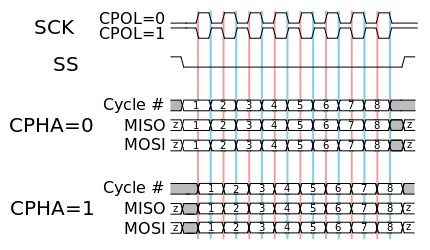
\includegraphics[width=1.0\linewidth]{SPI_timing}
}
\headerbox{Acknowledgements}{name=acknowledgements,column=0,below=joystick}{
	This research was supported by Professor Bill and Vitor Chao(a member of another team). The major information about fundamental of the CPU and PPU are obtained from http://wiki.nesdev.com. The supports are gratefully acknowledged.
}

\headerbox{High Level Architecture}{name=high_level_arch,span=2,column=1,row=0}{
	The code of the game are stored in \textbf{PROM}. The CPU can access both PROM and \textbf{PRAM} at run time. The pixel information of both background and sprites are stored in \textbf{VROM} and the VROM are combined of many tiles with size of 8 by 8 pixels. 
	The \textbf{index}\&\textbf{color} data of background are stored in \textbf{VRAM}, while sprites' are stored in \textbf{OAM}(also \textbf{coordinate}). The CPU creates the data and transfers them to the PPU through registers or \textbf{DMA}.
	The VGA signal generator creates the \textbf{Vsync}(60 times per second) and \textbf{Hsync}(480=240*2 times per frame) signal, and fetchs data from a double scanline buffer, in which the PPU put the data at first.

The figure below show the hight level architecture of our NES model
(red edge: index/address/trigger; green edge: data; gray: ROM; blue: RAM; bg\&sp are the abbreviation of background\&sprite).\\
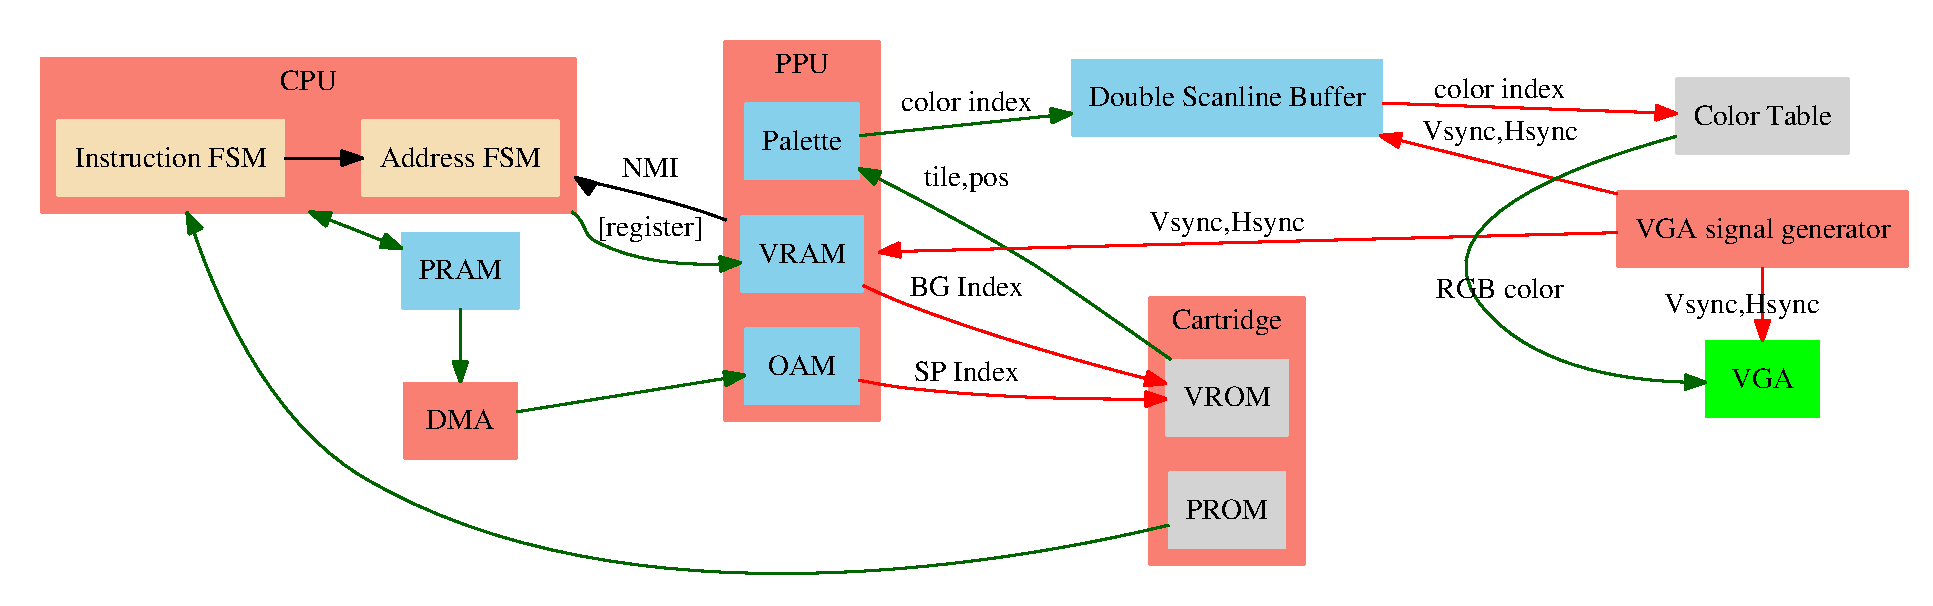
\includegraphics[width=1.0\linewidth]{high_level_arch_of_nes}
The process of creating a frame of image starts from trigger of NMI signal, the details of timing of each frame are demostrated here.\\
\\
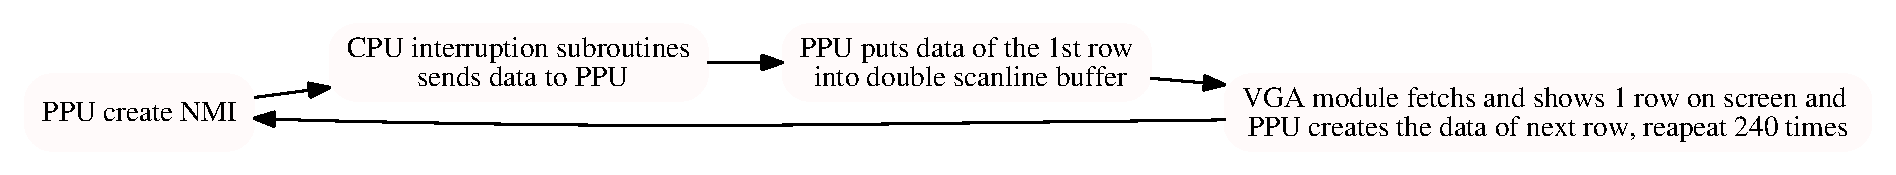
\includegraphics[width=1.0\linewidth]{time}
}

\headerbox{Introduction of the CPU 6502}{name=cpu_fsm,span=2,column=1,below=high_level_arch}{
%The following figure show all the useful instructions of CPU 6502.\\ 
	There are \textbf{56} different instructions in CPU 6502, we implemnt \textbf{54} of them, since we found BIT and BRK never occur in the C++ emulator of the Tank1990.\\ 
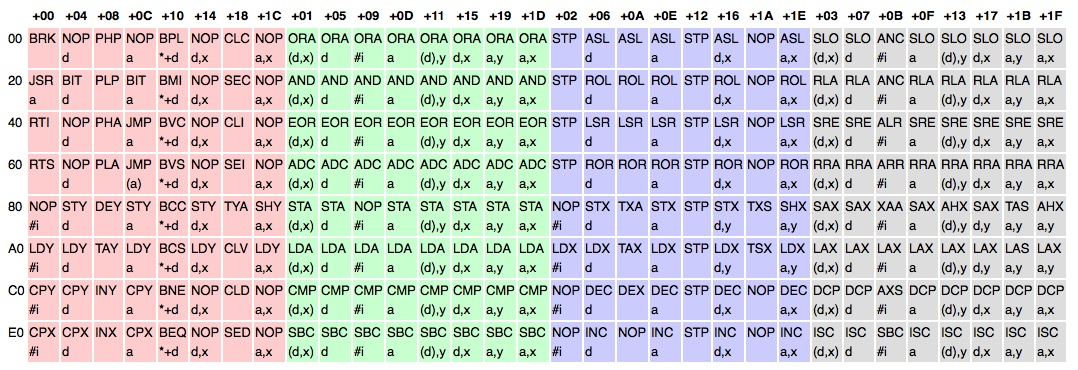
\includegraphics[width=1.0\linewidth]{ins}
	Instructions need operands to work on. There are various ways(addressing modes) of indicating where the processor is to get these operands. The 6502 offers \textbf{11} modes. The following figure demostrate 2 FSMs and their interfaces built in our CPU.
\\
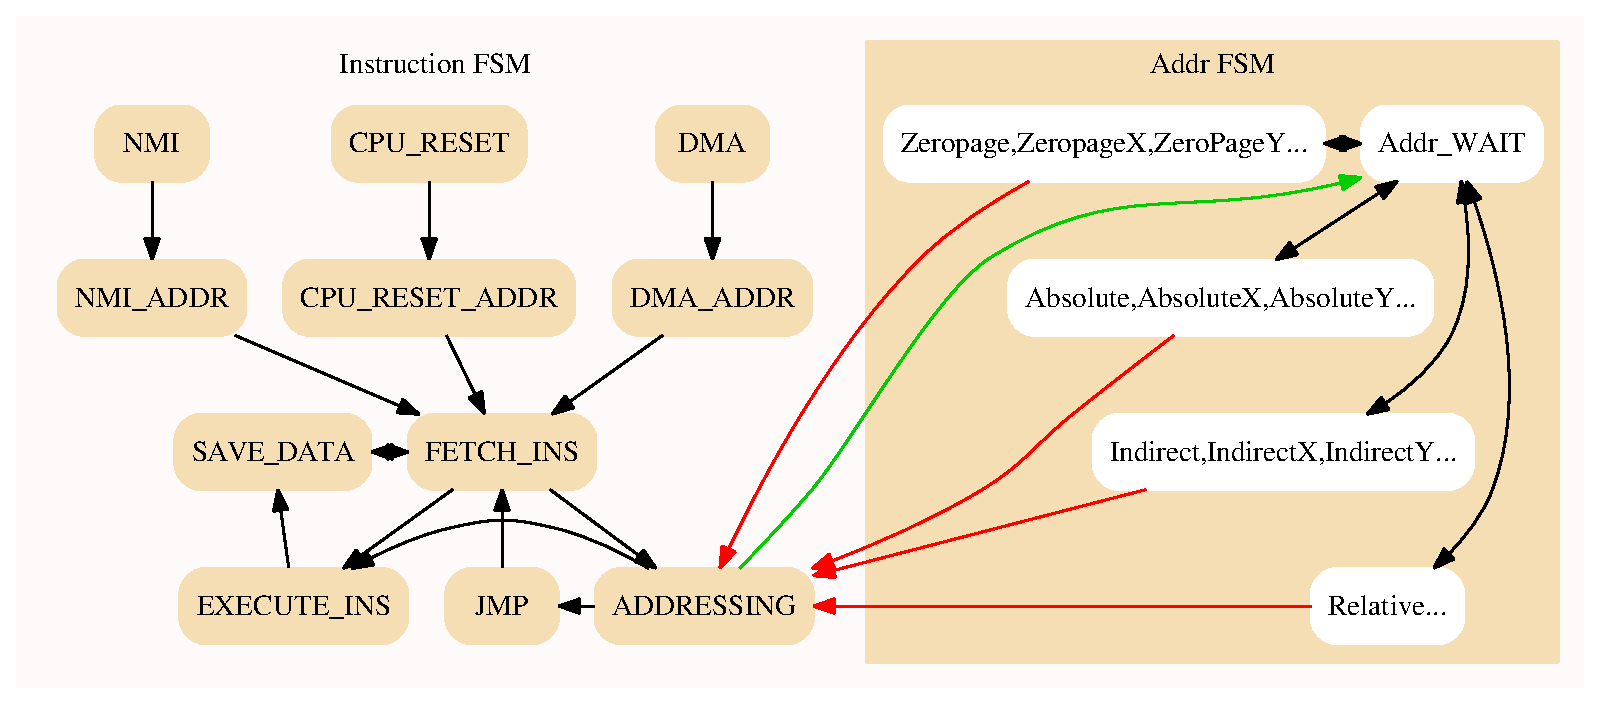
\includegraphics[width=1.0\linewidth]{cpu_fsm}
}

\headerbox{Framework of the PPU}
%{name=ppu_vga,span=2,column=1,below=cpu_fsm,above=bottom}{
{name=ppu_vga,span=2,column=1,below=cpu_fsm}{
The PPU is responsible for using the data sent from the CPU to construct the image(240*256) of the background and sprites. Here is 4 FSMs built in our PPU, we can consider the Control FSM is the master of the Background FSM and Sprite FSM, and these two FSM are both the master of the Palette FSM.([...] beside an edge indicates a counter).\\
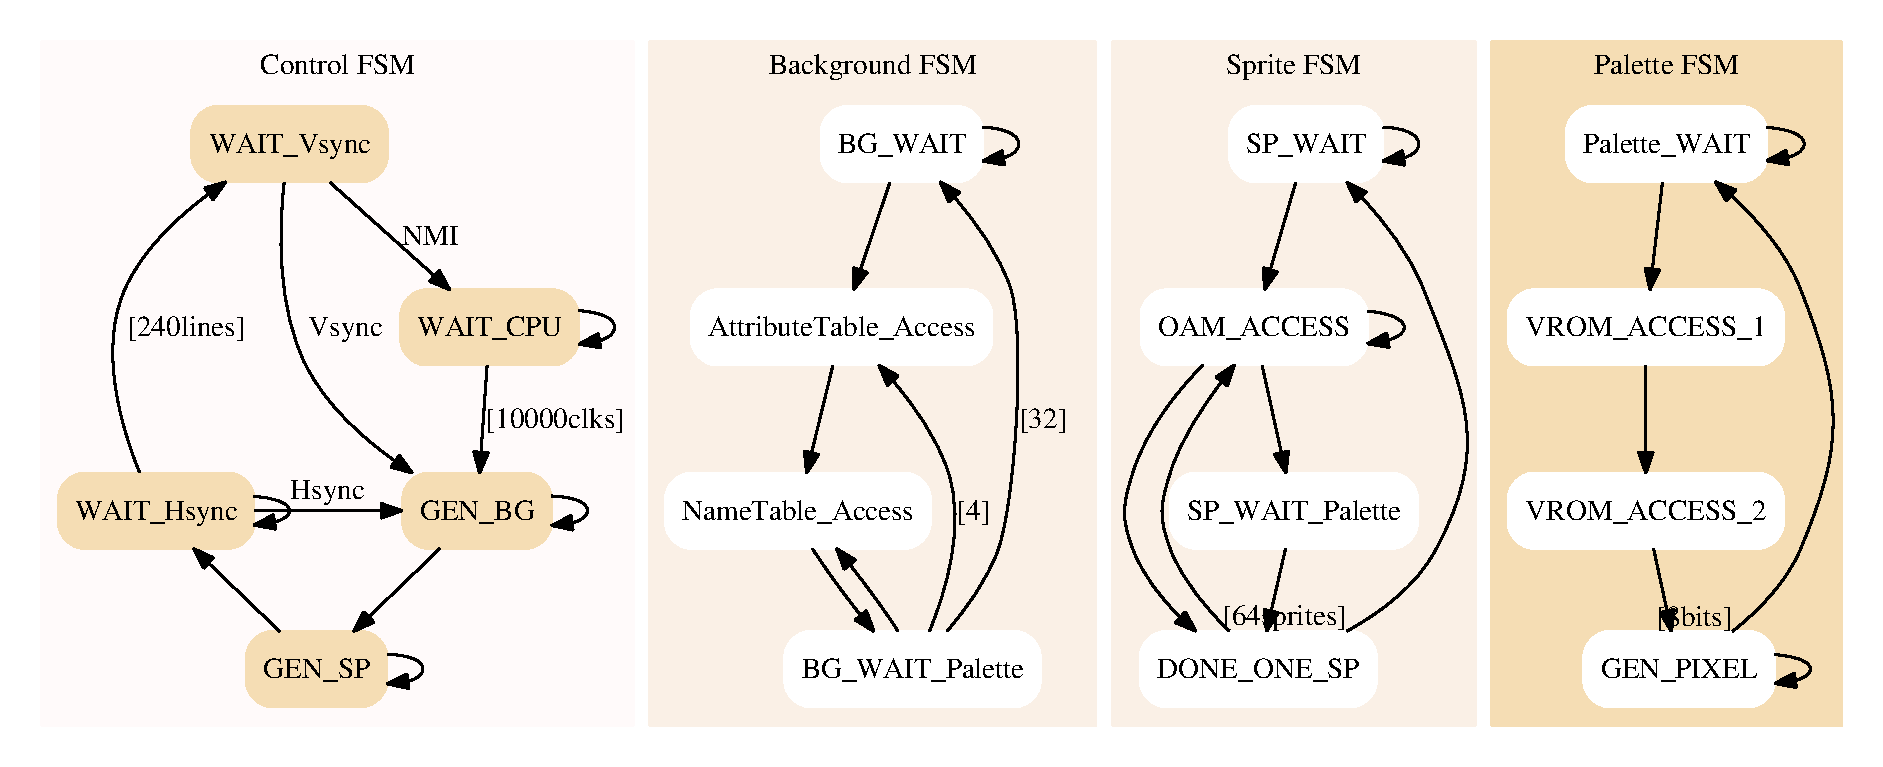
\includegraphics[width=1.0\linewidth]{ppu_fsm}
}

\end{poster}
\end{document}
